\documentclass[a4paper, 12pt]{article}
\usepackage[utf8]{inputenc}
\usepackage[lmargin=3cm, tmargin=3cm, rmargin=2cm, bmargin=2cm]{geometry}
\usepackage[onehalfspacing]{setspace}
\usepackage[T1]{fontenc}
\usepackage[brazil]{babel}

%%%\usepackage{amssymb, amsmath, mathptmx}%bigominus

\usepackage{wasysym}%male and female

\usepackage{graphicx, graphics, xcolor, comment, enumerate, multirow, multicol, indentfirst}

\usepackage{amsmath, amsthm, amsfonts, amssymb, dsfont, mathtools}
\everymath{\displaystyle} 

\usepackage{blindtext}

\usepackage[round]{natbib}
\bibliographystyle{apalike}

\usepackage{hyperref}

%Code packages:
\usepackage{listings}
\usepackage{xcolor}

%New colors defined below
\definecolor{codegreen}{rgb}{0,0.6,0}
\definecolor{codegray}{rgb}{0.5,0.5,0.5}
\definecolor{codepurple}{rgb}{0.58,0,0.82}
\definecolor{backcolour}{rgb}{0.95,0.95,0.92}

%Code listing style named "mystyle"
\lstdefinestyle{mystyle}{
  backgroundcolor=\color{backcolour},   commentstyle=\color{codegreen},
  keywordstyle=\color{magenta},
  numberstyle=\tiny\color{codegray},
  stringstyle=\color{codepurple},
  basicstyle=\ttfamily\footnotesize,
  breakatwhitespace=false,         
  breaklines=true,                 
  captionpos=b,                    
  keepspaces=true,                 
  numbers=left,                    
  numbersep=5pt,                  
  showspaces=false,                
  showstringspaces=false,
  showtabs=false,                  
  tabsize=2
}

%"mystyle" code listing set
\lstset{style=mystyle}

\title{Projeto 5: Como o Google Ordena as Páginas}
\author{
  Herberth Luan Vieira Oliveira\\
  \texttt{12559110}
  \and
  Juliana de Abreu Faria\\
  \texttt{10336275}
  \and
  Victor Viana de Oliveira Matos\\
  \texttt{11810821}
  \and
  Vinícius da Costa Collaço\\
  \texttt{11811012}
  \and
  Vitor Sillos Alonso\\
  \texttt{9506935}
}

\begin{document}

\maketitle

\section{Exercício 1}

Seja a matriz $\mathrm{M}$ da seguinte forma:

$$\mathrm{M}=\begin{pmatrix}
m_{11}&m_{12}&\dots &m_{1n}\\
m_{21}&m_{22}&\dots &m_{2n}\\
\vdots &\vdots &\ddots &\vdots \\
m_{n1}&m_{n2}&\dots &m_{nn}
\end{pmatrix}$$

Se $\mathrm{M}$ satisfaz as hipóteses do teorema 1 então temos as seguintes relações:

$$\begin{cases}
m_{11}+m_{21}+\dots +m_{n1}=1\\
m_{12}+m_{22}+\dots +m_{n2}=1\\
\ \ \ \ \ \ \ \ \ \ \ \ \ \vdots \\
m_{1n}+m_{2n}+\dots +m_{nn}=1
\end{cases}$$

Seja o vetor $\mathrm{y}$ da seguinte forma:

$$\mathrm{y}=\begin{pmatrix}
y_1\\
y_2\\
\vdots \\
y_n
\end{pmatrix}$$

Sendo o vetor $\mathrm{y}$ normalizado, temos que:

$$y_1+y_2+\dots +y_n=1$$

Fazendo $\mathrm{z}=\mathrm{M}\mathrm{y}$, temos que:

$$\mathrm{z}=\begin{pmatrix}
m_{11}&m_{12}&\dots &m_{1n}\\
m_{21}&m_{22}&\dots &m_{2n}\\
\vdots &\vdots &\ddots &\vdots \\
m_{n1}&m_{n2}&\dots &m_{nn}
\end{pmatrix}\begin{pmatrix}
y_1\\
y_2\\
\vdots \\
y_n
\end{pmatrix}$$

$$\mathrm{z}=\begin{pmatrix}
m_{11}\cdot y_1+m_{12}\cdot y_2+\dots +m_{1n}\cdot y_n\\
m_{21}\cdot y_1+m_{22}\cdot y_2+\dots +m_{2n}\cdot y_n\\
\vdots \\
m_{n1}\cdot y_1+m_{n2}\cdot y_2+\dots +m_{nn}\cdot y_n
\end{pmatrix}$$

Representando a soma de todos os elementos do vetor $\mathrm{z}$ por $S$, temos que:

\begin{footnotesize}
$$S=\left(m_{11}y_1+m_{12}y_2+\dots +m_{1n}y_n\right)+\left(m_{21}y_1+m_{22}y_2+\dots +m_{2n}y_n\right)+\dots +\left(m_{n1}y_1+m_{n2}y_2+\dots +m_{nn}y_n\right)$$
\end{footnotesize}$$S=\left(m_{11}+m_{21}+\dots+m_{n1}\right)y_1+\left(m_{12}+m_{22}+\dots+m_{n2}\right)y_2+\dots +\left(m_{1n}+m_{2n}+\dots+m_{nn}\right)y_n$$

Sabemos que $m_{11}+m_{21}+\dots+m_{n1}=1$, $m_{12}+m_{22}+\dots+m_{n2}=1$ e $m_{1n}+m_{2n}+\dots+m_{nn}=1$, então:

$$S=\left(1\right)y_1+\left(1\right)y_2+\dots +\left(1\right)y_n$$
$$S=y_1+y_2+\dots +y_n$$

Como visto acima $y_1+y_2+\dots +y_n=1$, então:

$$\boxed{\ \ S=1\ \ }$$

Portando está provado que a soma das entradas de $\mathrm{z}$ é igual a 1, então $\mathrm{z}$ é um vetor \textbf{normalizado}.

Também, é fácil verificar que todos as entradas de $\mathrm{z}$ são \textbf{positivas}, já que provém de somas e multiplicações de números positivos, pois todas as entradas de $\mathrm{M}$ e $\mathrm{y}$ são positivas.\\\\\\

\section{Exercício 2}
\subsection{Demonstração 1}
Sendo a matriz $\mathrm{S}$ da seguinte forma:

$$\mathrm{S}=\begin{pmatrix}
\frac{1}{n}&\frac{1}{n}&\dots &\frac{1}{n}\\
\frac{1}{n}&\frac{1}{n}&\dots &\frac{1}{n}\\
\ \vdots &\ \vdots &\ddots &\ \vdots \\
\frac{1}{n}&\frac{1}{n}&\dots &\frac{1}{n}
\end{pmatrix}$$


Então pela definição da matriz $\mathrm{M}$, temos que: 

$$\mathrm{M}=\left(1-m\right)\mathrm{A}+m\begin{pmatrix}
\frac{1}{n}&\frac{1}{n}&\dots &\frac{1}{n}\\
\frac{1}{n}&\frac{1}{n}&\dots &\frac{1}{n}\\
\ \vdots &\ \vdots &\ddots &\ \vdots \\
\frac{1}{n}&\frac{1}{n}&\dots &\frac{1}{n}
\end{pmatrix}$$

Multiplicando por $\mathrm{y}$ (pela direita) os dois lados da equação matricial acima temos: 

$$\mathrm{My}=\left(1-m\right)\mathrm{Ay}+m\begin{pmatrix}
\frac{1}{n}&\frac{1}{n}&\dots &\frac{1}{n}\\
\frac{1}{n}&\frac{1}{n}&\dots &\frac{1}{n}\\
\ \vdots &\ \vdots &\ddots &\ \vdots \\
\frac{1}{n}&\frac{1}{n}&\dots &\frac{1}{n}
\end{pmatrix}\begin{pmatrix}
\frac{1}{n}\\
\frac{1}{n}\\
\ \vdots \\
\frac{1}{n}
\end{pmatrix}$$

Desenvolvendo a multiplicação matricial temos:

$$\mathrm{My}=\left(1-m\right)\mathrm{Ay}+m\begin{pmatrix}
\frac{1}{n^2}+\frac{1}{n^2}+\dots +\frac{1}{n^2}\\
\frac{1}{n^2}+\frac{1}{n^2}+\dots +\frac{1}{n^2}\\
\vdots \\
\frac{1}{n^2}+\frac{1}{n^2}+\dots +\frac{1}{n^2}
\end{pmatrix}$$

$$\mathrm{My}=\left(1-m\right)\mathrm{Ay}+m\begin{pmatrix}
\frac{n}{n^2}\\
\frac{n}{n^2}\\
\vdots \\
\frac{n}{n^2}
\end{pmatrix}$$

Por fim, obtemos a igualdade pedida:

$$\boxed{\ \ \mathrm{My}=\left(1-m\right)\mathrm{Ay}+m\begin{pmatrix}
\frac{1}{n}\\
\frac{1}{n}\\
\vdots \\
\frac{1}{n}
\end{pmatrix}\ \ }$$

\subsection{Demonstração 2}

Como visto anteriormente, por definição a matriz $\mathrm{M}$ é data por:

$$\mathrm{M}=\left(1-m\right)\mathrm{A}+m\begin{pmatrix}
\frac{1}{n}&\frac{1}{n}&\dots &\frac{1}{n}\\
\frac{1}{n}&\frac{1}{n}&\dots &\frac{1}{n}\\
\ \vdots &\ \vdots &\ddots &\ \vdots \\
\frac{1}{n}&\frac{1}{n}&\dots &\frac{1}{n}
\end{pmatrix}$$

Multiplicando pelo vetor $\mathrm{y}$ (pela direita) em ambos os lados da equação matricial acima tem-se:

$$\mathrm{My}=\left(1-m\right)\mathrm{Ay}+m\begin{pmatrix}
\frac{1}{n}&\frac{1}{n}&\dots &\frac{1}{n}\\
\frac{1}{n}&\frac{1}{n}&\dots &\frac{1}{n}\\
\ \vdots &\ \vdots &\ddots &\ \vdots \\
\frac{1}{n}&\frac{1}{n}&\dots &\frac{1}{n}
\end{pmatrix}\begin{pmatrix}
y_1\\
y_2\\
\ \vdots \\
y_n
\end{pmatrix}$$

Desenvolvendo a multiplicação de matrizes:

$$\mathrm{My}=\left(1-m\right)\mathrm{Ay}+m\begin{pmatrix}
\frac{y_1}{n}+\frac{y_2}{n}+\dots +\frac{y_n}{n}\\
\ \frac{y_1}{n}+\frac{y_2}{n}+\dots +\frac{y_n}{n}\\
\vdots \\
\frac{y_1}{n}+\frac{y_2}{n}+\dots +\frac{y_n}{n}
\end{pmatrix}$$

Colocando os valores $1/n$ em evidência:

$$\mathrm{My}=\left(1-m\right)\mathrm{Ay}+m\begin{pmatrix}
\frac{1}{n}\left(y_1+y_2+\dots +y_n\right)\\
\ \frac{1}{n}\left(y_1+y_2+\dots +y_n\right)\\
\vdots \\
\frac{1}{n}\left(y_1+y_2+\dots +y_n\right)
\end{pmatrix}$$

Como todas as entradas de $\mathrm{y}$ somam 1, isto é, $y_1+y_2+\dots +y_n=1$, então por fim chegamos ao mesmo resultado encontrado anteriormente:

$$\boxed{\ \ \mathrm{My}=\left(1-m\right)\mathrm{Ay}+m\begin{pmatrix}
\frac{1}{n}\\
\frac{1}{n}\\
\vdots \\
\frac{1}{n}
\end{pmatrix}\ \ }$$

\section{Exercício 3}
\subsection{Criação da Matriz de Ligação}
Para a criação da matriz A partiremos do seguinte grafo:

\begin{center}
    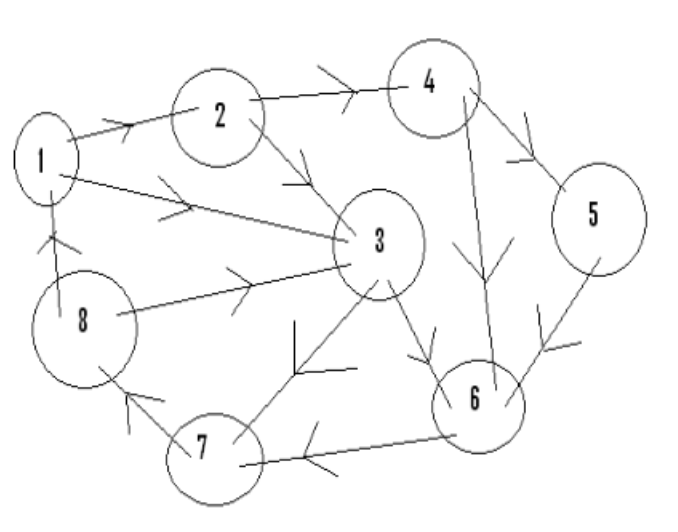
\includegraphics[width=16cm]{esquema.PNG}
     Representação esquemática para o teste do Exercício 3
    
\end{center}

A partir da figura, podemos escrever as equações para cada site, com pesos baseados para quantos sites o site referencia, e quantos sites referencial um determinado site. 

$$\begin{cases}
x_1 = x_8/2\\
x_2 = x_1/2\\
x_3 = x_1/2 + x_2/2 + x_8/2\\
x_4 = x_2/2 \\
x_5 = x_4/2\\
x_6 = x_3/2 + x_4/2 + x_5/1\\
x_7 = x_3/2 + x_6/1\\
x_8 = x_7/1
\end{cases}$$

O sistema linear pode então ser escrita em forma matricial da seguinte maneira:

$$\begin{pmatrix}
x_1\\
x_2\\
x_3\\
x_4\\
x_5\\
x_6\\
x_7\\
x_8
\end{pmatrix}=\begin{pmatrix}
0 & 0 & 0 & 0 & 0 & 0 & 0 & 1/2\\
1/2 & 0 & 0 & 0 & 0 & 0 & 0 & 0\\
1/2 & 1/2 & 0 & 0 & 0 & 0 & 0 & 1/2\\
0 & 1/2 & 0 & 0 & 0 & 0 & 0 & 0\\
0 & 0 & 0 & 1/2 & 0 & 0 & 0 & 0\\
0 & 0 & 1/2 & 1/2 & 1 & 0 & 0 & 0\\
0 & 0 & 1/2 & 0 & 0 & 1 & 0 & 0\\
0 & 0 & 0 & 0 & 0 & 0 & 1 & 0
\end{pmatrix}\cdot\begin{pmatrix}
x_1\\
x_2\\
x_3\\
x_4\\
x_5\\
x_6\\
x_7\\
x_8
\end{pmatrix}
$$
Temos então a nossa matriz de ligação (A), podemos escreve-la em um array para o uso do nosso algoritmo. Com auxílio da biblioteca numpy do python.

\begin{lstlisting}[language=Python, caption = Matriz de Ligação A]
import numpy as np

A = np.array([[0, 0, 0, 0, 0, 0, 0, 1/2],
             [1/2, 0, 0, 0, 0, 0, 0, 0],
             [1/2, 1/2, 0, 0, 0, 0, 0, 1/2],
             [0, 1/2, 0, 0, 0, 0, 0, 0],
             [0, 0, 0, 1/2, 0, 0, 0, 0],
             [0, 0, 1/2, 1/2, 1, 0, 0, 0],
             [0, 0, 1/2, 0, 0, 1, 0, 0],
             [0, 0, 0, 0, 0, 0, 1, 0]]              
              )
\end{lstlisting}

\subsection{Matriz pertubada}
A matriz de ligação criada a partir da figura, possui a soma das linhas igual à 1, garantindo que $Ax=x$, tenha solução, porém podemos perturbar essa matriz com um valor pequeno para termos uma matriz perturbada com as mesmas características da matriz de ligação, sem ter valores zerados nela. Pois tendo valores nulos, não são satisfeitas as hipóteses do teorema de Perron-Frobenius.

Substituimos então A pela matriz perturbada 

$$M = (1-m)A +mS$$

onde 0< m <1 e S é a matriz n x n com todas as entradas iguais a 1/n:

podemos então criar a matriz M da seguinte maneira:

\begin{lstlisting}[language=Python, caption=Matriz M]
  n = A.shape[1] #matriz de ligacao NxN
  S = np.full((n,n),(1/n))
  M = (1-m)*A + m*S
\end{lstlisting}

Essa correção feita na matriz A torna todas as entradas de M estritamente positivas e a soma dos elementos em cada coluna continua sendo igual a 1. Para todo m entre 0 e 1.

\subsection{Método das Potências}
Podemos então resolver o sistema linear pelo método das potências\citep{anton}, dado por:

$$x^{(k)} = Mx^{(k-1)}$$

Se a matriz M satisfaz as hipóteses do Teorema de Perron-Frobenius, $x^{(x)}$ converge para o autovetor normalizado associado ao autovalor 1 com taxa c.

\begin{lstlisting}[language=Python, caption=Método das Potências]
def MetodoPotencias(M,x0,k=50):
  x1 = M @ x0 #multiplicacao de matrizes, @ equivale ao np.dot
  for i in range(k-1):
    x1 = M @ x1
  return x1
\end{lstlisting}

O valor converge rápido, quanto mais iterações mais próximo do valor real. No programa criado foi adotado arbitrariamente um número padrão de 50 iterações.

\subsubsection{Exemplo do Algoritimo do Método das Potências}

\begin{center}
    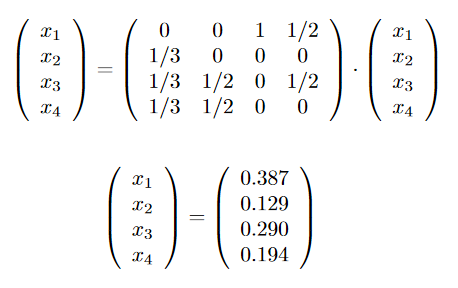
\includegraphics[width=9cm]{Exemplo_pot.PNG}
    
    Exemplo 1
\end{center}

utilizando o algoritimo criado para resolver o problema temos:

\begin{lstlisting}[language=Python, caption=Resolução do Exemplo 1 pelo algoritmo]
#Resolucao Intro
A_intro = np.array([[0, 0, 1, 1/2],
                    [1/3, 0, 0, 0],
                    [1/3, 1/2, 0, 1/2],
                    [1/3, 1/2, 0, 0]])
n = A_intro.shape[1]
x0 = np.full((n,1),(1/n))
MetodoPotencias(A_intro, x0).round(3)
\end{lstlisting}

\begin{center}
    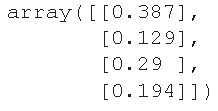
\includegraphics[width=5cm]{saida_ex1.PNG}
    
    Saída do Exemplo 1 
\end{center}

A saída obtida corresponde ao exemplo, a matriz ligação do exemplo não é uma matriz perturbada, porém converge à uma resolução.

\subsection{Taxa c e cálculo do erro}

O método das potências converge o resultado com uma taxa c dada por:

$$c = max_{1\leq j \leq n}\left|{1-2 *(min_{1\leq i \leq n} M_{ij})} \right|$$

assim podemos calcular o c com a seguinte função:

\begin{lstlisting}[language=Python, caption=Cálculo da taxa c]
def calculo_c(M):
  #minimo de cada coluna
  min_col = np.amin(M, axis=1)
  c = max(abs(1-2*min_col))
  return c
\end{lstlisting}

tendo a taxa c calculada podemos calcular a estimativa do erro a posteriori por:

$$\|x - x^{(k)}\|\leq \frac{c}{1-c}\|x^{(k)}-x^{(k-1)}\|$$

onde x é o autovetor normalizado.
Em python podemos normalizar um vetor com auxílio da biblioteca numpy com a função "np.linalg.norm"

\subsection{Cálculo do Vetor dos Pesos Normalizado}
Tendo a matriz de ligação, a matriz perturbada, c e a estimativa do erro. Podemos então criar o algoritmo para ordenar as "páginas".

\begin{lstlisting}[language=Python, caption=Algoritmo para a ordenação de páginas até um certo erro]
def OrdenaPaginas(A, x0, m=0.15, erro=1e-5):
  n = A.shape[1] #matriz de ligacao NxN
  S = np.full((n,n),(1/n))
  M = (1-m)*A + m*S
  e = erro + 1 #erro inicial para entrar no loop
  cnt = 0 #contador inicial
  c = calculo_c(M)
  xk_1 = x0 

  while e > erro:
    xk = M @ xk_1
    e = c/(1-c)*np.linalg.norm(xk - xk_1)
    xk_1 = xk 
    cnt += 1
  
  print(f'c = {c}')
  print(f'Vetor dos pesos normalizado:\n{xk}\nApos {cnt} iteracoes ', end='')
  print(f'com erro menor que {erro}')
\end{lstlisting}

\begin{center}
    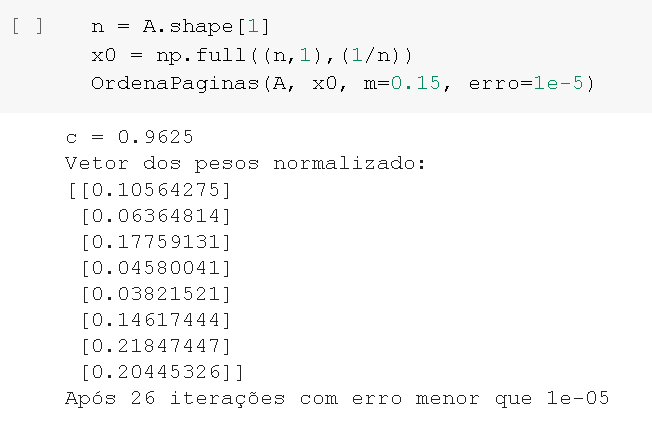
\includegraphics[width=16cm]{Saida_ordena2.PNG}
    
    Saída do programa para o problema do exercício 3
\end{center}

Após 26 iterações conseguimos a saída com erro menor que $10^{-5}$ e $c=0.9625$. Podemos observar pelo resultado que a "página" mais importante, no exemplo, é a página 6, seguida pela 7 e em terceiro lugar a página 3. Interessante observar que a página 3 é referenciada mais vezes que a página 7, porém a página 7 acaba tendo mais relevância por ser referenciada por páginas mais relevantes, no caso a 6 e a 3.

\section{Código Fonte}
\href{https://colab.research.google.com/drive/1nWHHrDlD-4zl05NxqaqwESCP_GQQOw_S?usp=sharing}{https://colab.research.google.com/drive/1nWHHrDlD-4zl05NxqaqwESCP\_GQQOw\_S?}

Código criado em Python, com o Jupyter Notebook no Google Colaboratory.

\section{Considerações Finais}

O projeto teve o intuito de observar a maneira com que diferentes paginas da web são relacionadas entre si através de um algorítimo de um sistema de procura. Para tanto, primeiro observou-se o Teorema de Perron-Frobenius, na qual considerando-se uma matriz M n x n com todos os seus elementos positivos e cujas colunas somam 1, temos que:

\begin{itemize}
   \item 1 será o autovalor de maior módulo de M;
   \item seu auto-espaço é unidimensional;
   \item o autovetor normalizado só tem entradas estritamente positivas.
 \end{itemize}

Isto posto, foi desenvolvido um programa em python que buscou encontrar as relações entre as paginas através do método das potências. Primeiramente, utilizou-se um valor para m igual a 0,15. Em seguida, calculou-se uma matriz perturbada para que não houvessem valores nulos e assim fossem respeitadas as hipóteses do teorema de Perron-Frobenius. Então, o sistema linear foi resolvido utilizando-se um numero arbitrário de 50 iterações.

No próximo passo, foram obtidas a taxa c e o cálculo do erro. A taxa c corresponde à taxa com o qual o método das potências converge ao resultado, e com ele foi possível obter a estimativa do erro. Por fim, foi aplicado o algorítimo e após 26 iterações  encontrou-se um valor c = 0.9625 e erro menor que $10^{(-5)}$.

Como observações, no exercício desenvolvido o grafo usado possuía poucas ligações, logo a matriz A possuía valores nulos em todas as colunas, fazendo com que o valor c fosse para um valor máximo. Em um caso com exemplos reais, talvez houvessem mais conexões e um valor menor para c, aumentando a complexidade do processamento.


\bibliography{ref.bib}

\end{document}